\let\negmedspace\undefined
\let\negthickspace\undefined
\documentclass[journal,12pt,onecolumn]{IEEEtran}
\usepackage{cite}
\usepackage{amsmath,amssymb,amsfonts,amsthm}
\usepackage{algorithmic}
\usepackage{graphicx}
\usepackage{textcomp}
\usepackage{xcolor}
\usepackage{txfonts}
\usepackage{listings}
\usepackage{enumitem}
\usepackage{mathtools}
\usepackage{gensymb}
\usepackage{comment}
\usepackage{caption}
\usepackage[breaklinks=true]{hyperref}
\usepackage{tkz-euclide} 
\usepackage{listings}
\usepackage{gvv}                                        
%\def\inputGnumericTable{}                                 
\usepackage[latin1]{inputenc}     
\usepackage{xparse}
\usepackage{color}                                            
\usepackage{array}                                            
\usepackage{longtable}                                       
\usepackage{calc}                                             
\usepackage{multirow}
\usepackage{multicol}
\usepackage{hhline}                                           
\usepackage{ifthen}                                           
\usepackage{lscape}
\usepackage{tabularx}
\usepackage{array}
\usepackage{float}
%\newtheorem{theorem}{Theorem}[section]
%\newtheorem{theorem}{Theorem}[section]
%\newtheorem{problem}{Problem}
%\newtheorem{proposition}{Proposition}[section]
%\newtheorem{lemma}{Lemma}[section]
%\newtheorem{corollary}[theorem]{Corollary}
%\newtheorem{example}{Example}[section]
%\newtheorem{definition}[problem]{Definition}

\begin{document}

\title{2.10.24}
\author{AI25BTECH11035 - SUJAL RAJANI}
% \maketitle
% \newpage
% \bigskip
%\begin{document}
{\let\newpage\relax\maketitle}
%\renewcommand{\thefigure}{\theenumi}
%\renewcommand{\thetable}{\theenumi}
% \newpage
% \bigskip
\textbf{Question}:
\\
 Let $\vec{x}$,$\vec{y}$ and $\vec{z}$ be three vectors each of magnitude $\sqrt 2$ and the angle between each pair of them is $\dfrac{\pi}{3}$. If $\vec{a}$ is a non-zero vector perpendicular to $\vec{x}$ and $\vec{y}$ x $\vec{z}$ and $\vec{b}$ is a non-zero vector perpendicular to $\vec{y}$ and $\vec{z}$ x $\vec{x}$, then
 \begin{enumerate}
 \begin{multicols}{2}
     \item  $\vec{b}$ = ($\vec{b}\cdot\vec{z}$)($\vec{z}-\vec{x}$)
      \item  $\vec{a}$ = ($\vec{a}.\vec{y}$)($\vec{y}-\vec{z}$)
       \item  $\vec{a}.\vec{b}$ = -($\vec{a}.\vec{y}$)($\vec{b}.\vec{z}$)
       \item  $\vec{a}$ = -($\vec{a}.\vec{y}$)($\vec{z}-\vec{y}$)
 \end{multicols} 
 \end{enumerate}
\\
solution :
\\
defining : triple vector product 
\begin{align*}
    (\vec{x}X(\vec{y} X \vec{z}))=(\vec{x}^\top \vec{z})\vec{y}-(\vec{x}^\top \vec{y})\vec{z}
\end{align*}
\\
as mentioned in the question : 
\begin{align*}
    ||\vec{x}||=\sqrt{2},
    ||\vec{y}||=\sqrt{2},
    ||\vec{z}||=\sqrt{2}
    \\
\vec{x}^\top\vec{y}=1,\vec{x}^\top\vec{z}=1,\vec{y}^\top\vec{z}=1
\end{align*}
If $\vec{a}$ is a non-zero vector perpendicular to $\vec{x}$ and $\vec{y}$ x $\vec{z}$ this implies :
\\
\begin{align*}
    \vec{a}^\top\vec{x}=0, \vec{a}^\top(\vec{y} X \vec{z})=0
\end{align*}
this implies that  $\vec{x}$ and $\vec{y} X \vec{z}$ lie in the same plane and their vector product is parallel to $\vec{a}$
\\
so the vector product of 
\\
\begin{align*}
    \vec{a}X(\vec{x}X(\vec{y} X \vec{z}))=0
\end{align*}

\begin{align*}
    \vec{x}^\top\vec{z}=1,\vec{x}^\top\vec{y}=1
    \\
    \vec{a}X(\vec{x}X(\vec{y} X \vec{z}))=(\vec{x}^\top\vec{z})(\vec{y}X\vec{a})-(\vec{x}^\top\vec{y})(\vec{z}X\vec{a)}=\vec{a}X(\vec{y}-\vec{z})
\end{align*}
as $\vec{a}$ is parallel to $\vec{y}-\vec{z}$ so we can say that :
\begin{align*}
    \vec{a}=k(\vec{y}-\vec{z})
\end{align*}
\\
k is a  constant
\\
If $\vec{b}$ is a non-zero vector perpendicular to $\vec{y}$ and $\vec{z}$ x $\vec{x}$ this implies :
\\

\begin{align*}
    \vec{b}^\top\vec{y}=0, \vec{b}^\top(\vec{z} X \vec{x})=0
\end{align*}
\\
this implies that  $\vec{x}$ and $\vec{y} X \vec{z}$ lie in the same plane and their vector product is parallel to $\vec{a}$
\\
so the vector product of 
\\
\begin{align*}
    \vec{b}X(\vec{y}X(\vec{z} X \vec{x}))=0
\end{align*}
\\

\\
\begin{align*}
\\
    \vec{x}^\top\vec{y}=1,\vec{z}^\top\vec{y}=1
    \\ 
    \vec{bX}(\vec{y}X(\vec{z} X \vec{x}))=(\vec{y}^\top\vec{x})(\vec{z}X\vec{b})-(\vec{y}^\top\vec{z})(\vec{x}X\vec{b})=\vec{b}X(\vec{z}-\vec{x})=0 
\end{align*}
as $\vec{b}$ is parallel to $\vec{z}-\vec{x}$ so we can say that :
\begin{align*}
    \vec{b}=m(\vec{z}-\vec{x})
\end{align*}
\\
m is a  constant
\\
now we check options one by one :
\\
\\
option (a)
\\
$\vec{b}$ = ($\vec{b}.\vec{z}$)($\vec{z}-\vec{x}$)
\\
we are putting b on both sides=
\\
 \begin{align*}
    m(\vec{z}-\vec{x})=( m(\vec{z}-\vec{x})^\top\vec{z})(\vec{z}-\vec{x}) 
    \\
    m(\vec{z}-\vec{x})=m(\vec{z}.\vec{z}-\vec{x}^\top\vec{z})(\vec{z}-\vec{x}) 
    \\
    \\
     m(\vec{z}-\vec{x})= m(\vec{z}-\vec{x})
 \end{align*}
 option A is correct . 
 \\
 option (b)
\\
$\vec{a}$ = ($\vec{a}^\top\vec{y}$)($\vec{y}-\vec{z}$)
\\
we are putting a on both sides=
\\
 \begin{align*}
   k(\vec{y}-\vec{z})=(k(\vec{y}-\vec{z})^\top\vec{y})(\vec{y}-\vec{z})
    \\
    k(\vec{y}-\vec{z})=(k(\vec{y}^\top\vec{y}-\vec{y}^\top\vec{z})(\vec{y}-\vec{z})
    \\
    \\
     k(\vec{y}-\vec{z})= k(\vec{y}-\vec{z})
 \end{align*}
 option B is correct .
\\  
 option (c)
\\
$\vec{a}^\top\vec{b}$ = -($\vec{a}^\top\vec{y}$)($\vec{b}^\top\vec{z}$)
\\
we are putting a and b on both sides=
\\
\begin{align*}
    k(\vec{y}-\vec{z})m(\vec{z}-\vec{x})=-( m(\vec{z}-\vec{x}).\vec{z})(k(\vec{y}-\vec{z})^\top\vec{y})
    \\
    -km=-km
\end{align*}
option C is correct  .
\\
option D is correct because option B is correct.
\\
for plotting we are assuming the position vector :
\\
\begin{align*}
    \vec x=\myvec{1\\1\\0},\vec y=\myvec{1\\0\\1},\vec z=\myvec{0\\1\\1},\vec a=\myvec{-1\\1\\0},\vec b=\myvec{-1\\0\\1}
\end{align*}



 \begin{figure}[H]
    \centering
    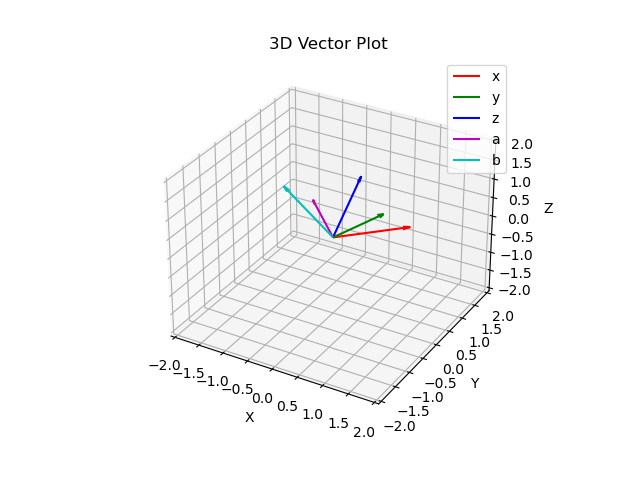
\includegraphics[width = 0.7\columnwidth]{figs/img.png}
    \caption*{}
    \label{figs}
\end{figure}

\end{document}